\documentclass{beamer}

% Theme choice
\usetheme{Madrid}

% Optional packages
\usepackage{graphicx} % For including images
\usepackage{amsmath}  % For math symbols and formulas
\usepackage{hyperref} % For hyperlinks
\usepackage{listings}
\usepackage{xcolor}
\usepackage[T1]{fontenc}

\lstdefinestyle{CStyle}{
  language=C,                    % Set the language to C
  basicstyle=\ttfamily\footnotesize\linespread{0.9}\tiny, % Set font style and size
  keywordstyle=\color{blue},      % Color of keywords
  commentstyle=\color{gray},      % Color of comments
  stringstyle=\color{red},        % Color of strings
  showstringspaces=false,         % Do not mark spaces in strings
  breaklines=true,                % Enable line breaks at appropriate places
  breakatwhitespace=false,        % Break lines at any character, not just whitespace
  numbers=left,                   % Show line numbers on the left
  numberstyle=\tiny\color{gray},  % Style for line numbers
  tabsize=4,                      % Set tab width
  keepspaces=true,                % Keep indentation spaces
  frame=single,                   % Add a border around the code
  aboveskip=0pt,                  % Reduce space above the code block
  belowskip=0pt,                   % Reduce space below the code block
  xleftmargin=7.5pt,                      % Add left padding (approx. 2.8mm or 10px)
  xrightmargin=15pt,                      % Add left padding (approx. 2.8mm or 10px)
}

% Title, author, date, and institute (optional)
\title[Parallel Programming. Parallelism practice]{Parallel Programming course. Parallelism practice}
\author{Obolenskiy Arseniy, Nesterov Alexander}
\institute{Nizhny Novgorod State University}

\date{\today} % or \date{Month Day, Year}

% Redefine the footline to display both the short title and the university name
\setbeamertemplate{footline}{
  \leavevmode%
  \hbox{%
    \begin{beamercolorbox}[wd=.45\paperwidth,ht=2.5ex,dp=1ex,leftskip=1em,center]{author in head/foot}%
        \usebeamerfont{author in head/foot}\insertshortinstitute % Displays the university name
    \end{beamercolorbox}%
    \begin{beamercolorbox}[wd=.45\paperwidth,ht=2.5ex,dp=1ex,leftskip=1em,center]{author in head/foot}%
      \usebeamerfont{author in head/foot}\insertshorttitle % Displays the short title
    \end{beamercolorbox}%
    \begin{beamercolorbox}[wd=.1\paperwidth,ht=2.5ex,dp=1ex,rightskip=1em,center]{author in head/foot}%
      \usebeamerfont{author in head/foot}\insertframenumber{} / \inserttotalframenumber
    \end{beamercolorbox}}%
  \vskip0pt%
}

\begin{document}

\begin{frame}
    \titlepage
\end{frame}

\begin{frame}{Contents}
    \tableofcontents
\end{frame}

\begin{frame}{Full list of tasks}
  \tiny
  \begin{itemize}
    \item Producer-Consumer Problem
    \item Readers-Writers Problem
    \item Dining Philosophers Problem
    \item Sleeping Barber Problem
    \item Broadcast (one-to-all communication)
    \item Reduce (all-to-one communication)
    \item Allreduce (all-to-one communication and broadcast)
    \item Scatter (generalized one-to-all communication)
    \item Gather (generalized all-to-one communication)
    \item Topology: Line
    \item Topology: Ring
    \item Topology: Star
    \item Topology: Torus Grid
    \item Topology: Hypercube
    \item Horizontal Strip Scheme
    \item Vertical Strip Scheme
    \item Horizontal Strip Scheme (only matrix A partitioned)
    \item Horizontal Strip Scheme for A, Vertical Strip Scheme for B
    \item Gaussian Method - Horizontal Strip Scheme
    \item Gaussian Method - Vertical Strip Scheme
    \item Gauss-Jordan Method
    \item Iterative Methods (Jacobi)
    \item Iterative Methods (Gauss-Seidel)
    \item Simple Iteration Method
    \item Bubble Sort (Odd-Even Transposition Sort)
    \item Image Smoothing
    \item Contrast Enhancement
  \end{itemize}
\end{frame}


\section{Tasks}

\begin{frame}{Tasks}
  Tasks in the course are split into the following subgroups:
  \begin{itemize}
    \item Classical Tasks of Parallel Programming
    \item Data Transfer Methods
    \item Topologies
    \item Matrix Multiplication
    \item Systems of Linear Algebraic Equations
    \item Sort
    \item Image Processing
  \end{itemize}
\end{frame}

\begin{frame}{Disclaimers}
  \begin{itemize}
    \item All matrices should be stored in linear arrays (not \texttt{std::vector<std::vector<int> >})
    \item Performance should be measured on big matrices/vectors
    \item Total execution time (per test) is more than 1 second
    \item Functionality should be preserved for wide range of processes count
  \end{itemize}
\end{frame}

\section{Classical Tasks of Parallel Programming}

\begin{frame}{Classical Tasks of Parallel Programming}
  \begin{itemize}
    \item Producer-Consumer Problem
    \item Readers-Writers Problem
    \item Dining Philosophers Problem
    \item Sleeping Barber Problem
  \end{itemize}
  Warning:
  There is different testing mechanism. Time is not measured for these tasks.
  Tasks are measured with big number of processes (16+, up to physical limit)
\end{frame}

\begin{frame}{Producer-Consumer Problem}
  We have multiple processes: \textbf{several producers and several consumers}.
  Producer produces the data, consumer needs to read it.

  The producer-consumer problem is a classic synchronization scenario where one or more producers generate data and place it into a buffer, and one or more consumers remove data from the buffer for processing. The challenge is to ensure that producers do not add data into a full buffer and consumers do not remove data from an empty buffer, all while maintaining data integrity and synchronization.

  In the context of MPI we can implement the producer-consumer problem by using message passing between processes.

  Source: \href{https://en.wikipedia.org/wiki/Producer–consumer_problem}{https://en.wikipedia.org/wiki/Producer–consumer\_problem}
\end{frame}

\begin{frame}{Readers-Writers Problem}
  Some processes may read and some may write, with the constraint that no process may access the shared resource for either reading or writing while another process is in the act of writing to it.

  A readers-writer lock is a data structure that solves one or more of the readers-writers problems.

  Source: \href{https://en.wikipedia.org/wiki/Readers–writers_problem}{https://en.wikipedia.org/wiki/Readers–writers\_problem}
\end{frame}

\begin{frame}{Dining Philosophers Problem}
  Five philosophers dine together at the same table. Each philosopher has their own plate at the table. There is a fork between each plate. The dish served is a kind of spaghetti which has to be eaten with two forks. Each philosopher can only alternately think and eat. Moreover, a philosopher can only eat their spaghetti when they have both a left and right fork. Thus two forks will only be available when their two nearest neighbors are thinking, not eating. After an individual philosopher finishes eating, they will put down both forks. The problem is how to design a regimen (a concurrent algorithm) such that any philosopher will not starve; i.e., each can forever continue to alternate between eating and thinking, assuming that no philosopher can know when others may want to eat or think (an issue of incomplete information).

  Source: \href{https://en.wikipedia.org/wiki/Dining_philosophers_problem}{https://en.wikipedia.org/wiki/Dining\_philosophers\_problem}
\end{frame}

\begin{frame}{Sleeping barber problem}
  Imagine a hypothetical barbershop with one barber, one barber chair, and a waiting room with n chairs (n may be 0) for waiting customers. The following rules apply:
  \begin{itemize}
    \item If there are no customers, the barber falls asleep in the chair
    \item A customer must wake the barber if he is asleep
    \item If a customer arrives while the barber is working, the customer leaves if all chairs are occupied and sits in an empty chair if it's available
    \item When the barber finishes a haircut, he inspects the waiting room to see if there are any waiting customers and falls asleep if there are none
  \end{itemize}

  Source: \href{https://en.wikipedia.org/wiki/Sleeping_barber_problem}{https://en.wikipedia.org/wiki/Sleeping\_barber\_problem}
\end{frame}

\section{Data Transfer Methods}

\begin{frame}{Data Transfer Methods}
  \begin{itemize}
    \item Broadcast (one-to-all communication)
    \item Reduce (all-to-one communication)
    \item Allreduce (all-to-one communication and broadcast)
    \item Scatter (generalized one-to-all communication)
    \item Gather (generalized all-to-one communication)
  \end{itemize}
\end{frame}

\begin{frame}{Data Transfer Methods: details}
  There is no specific task for this section. You should come up with your own:
  \begin{itemize}
    \item Requirement: Put the task you have chosen in the description
    \item Reference implementation: original MPI function
    \item Tasks size should be big. Broadcast should send more that one element (vector)
    \item Consider using binary trees to distribute data across different processes
  \end{itemize}
\end{frame}

\section{Topologies}

\begin{frame}{Topologies}
  \begin{itemize}
    \item Topology: Line
    \item Topology: Ring
    \item Topology: Star
    \item Topology: Torus Grid
    \item Topology: Hypercube
  \end{itemize}
  Warning:
  There is different testing mechanism. Time is not measured for these tasks.
  Tasks are measured with big number of processes (16+, up to physical limit)

  Data is transferred from process 0
\end{frame}

\begin{frame}{Line topology}
  \begin{figure}[h]
    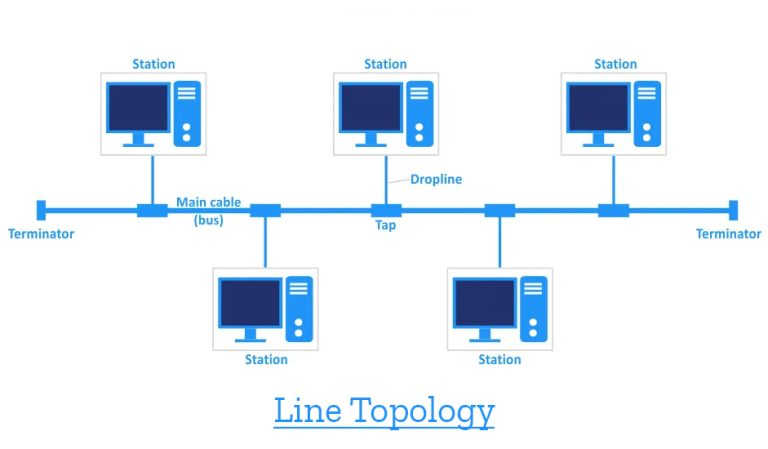
\includegraphics[width=1\textwidth]{images/line-topology.jpg}
  \end{figure}
\end{frame}

\begin{frame}{Ring topology}
  \begin{figure}[h]
    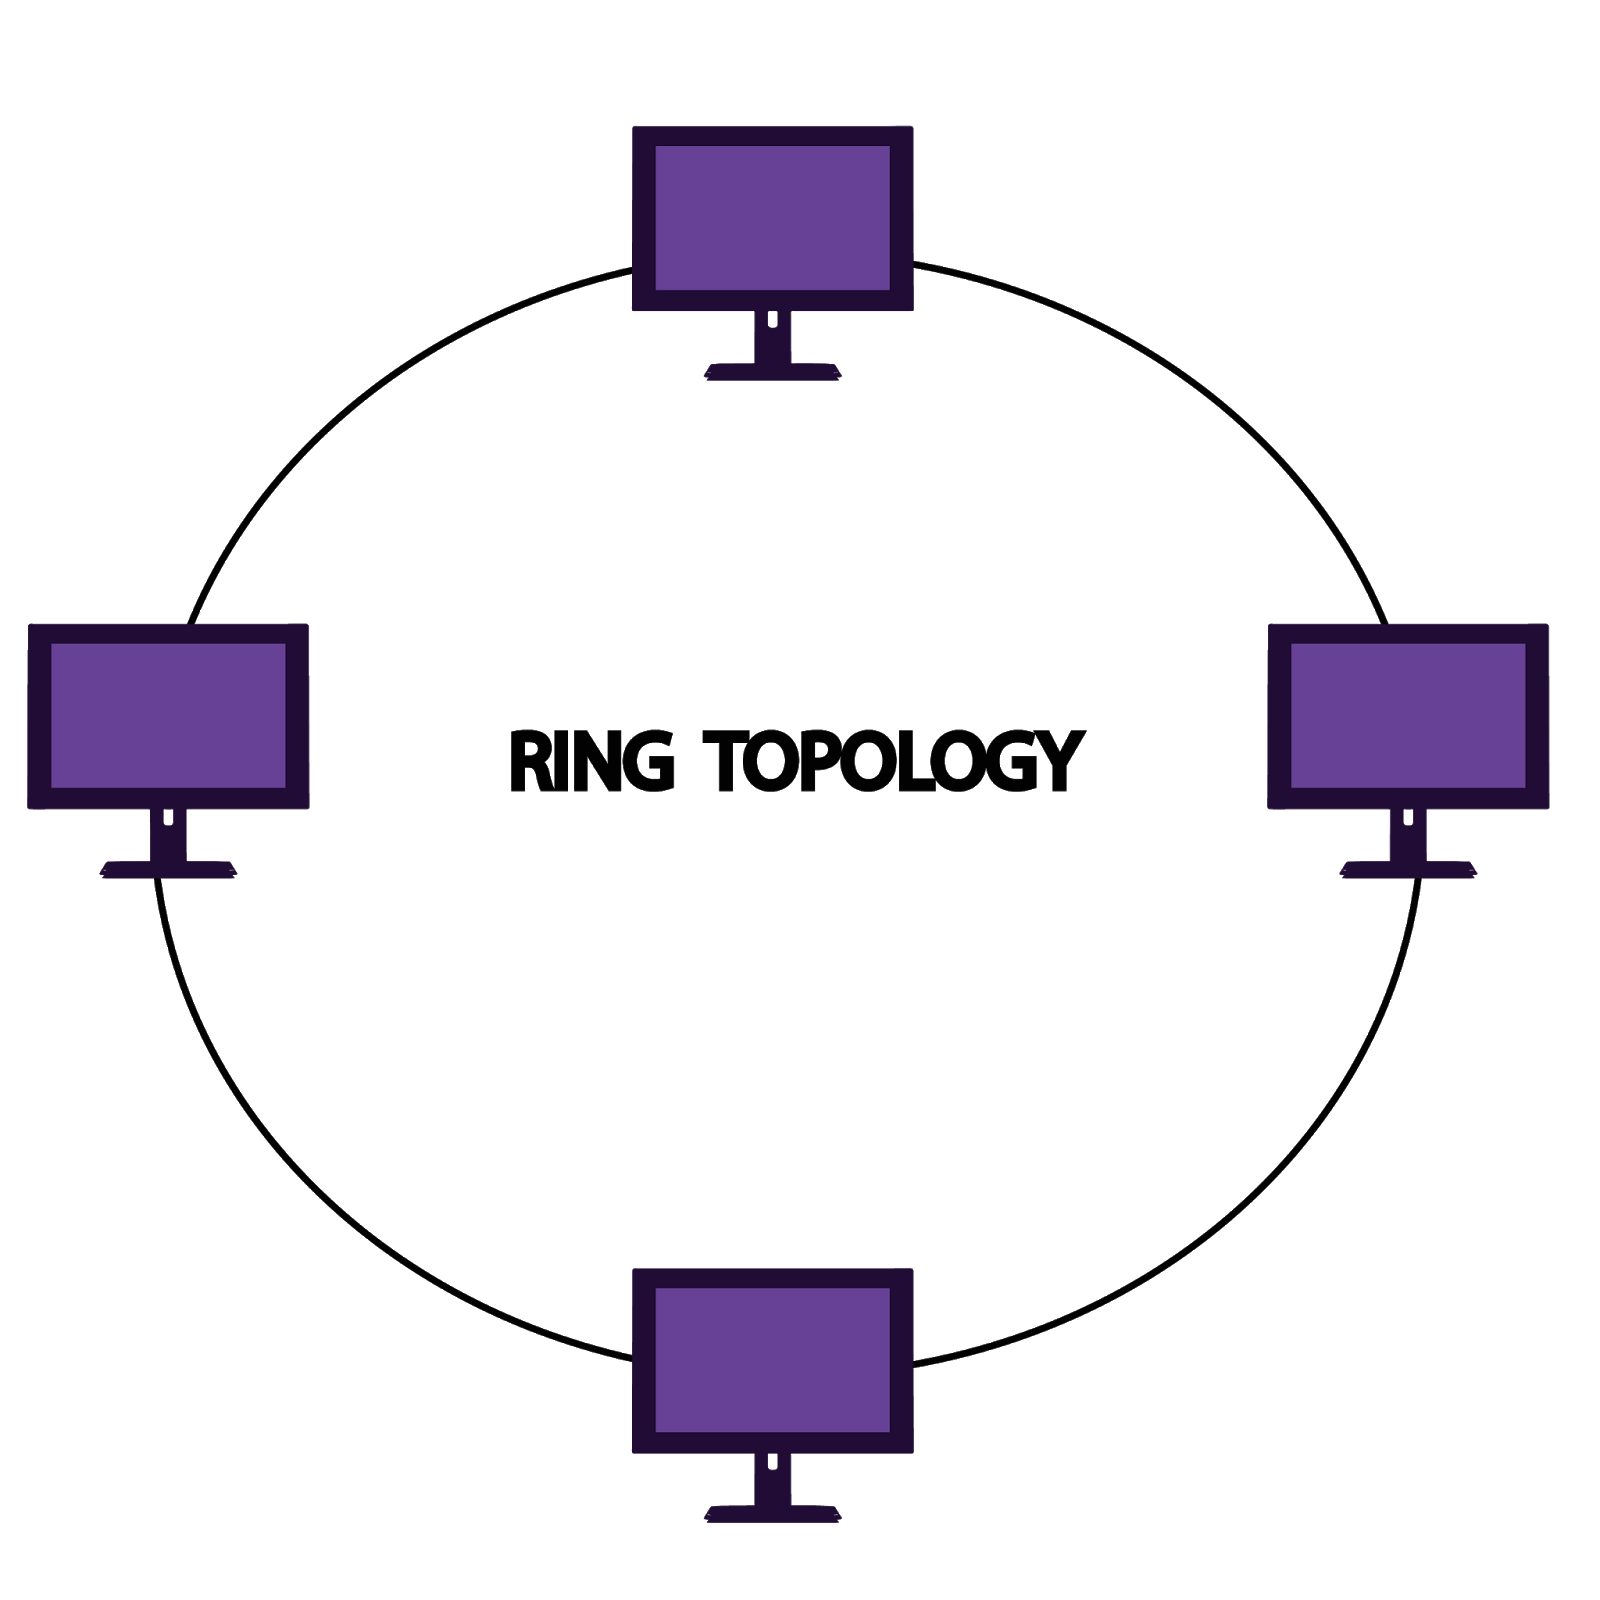
\includegraphics[width=0.65\textwidth]{images/ring-topology.png}
  \end{figure}
\end{frame}

\begin{frame}{Star topology}
  \begin{figure}[h]
    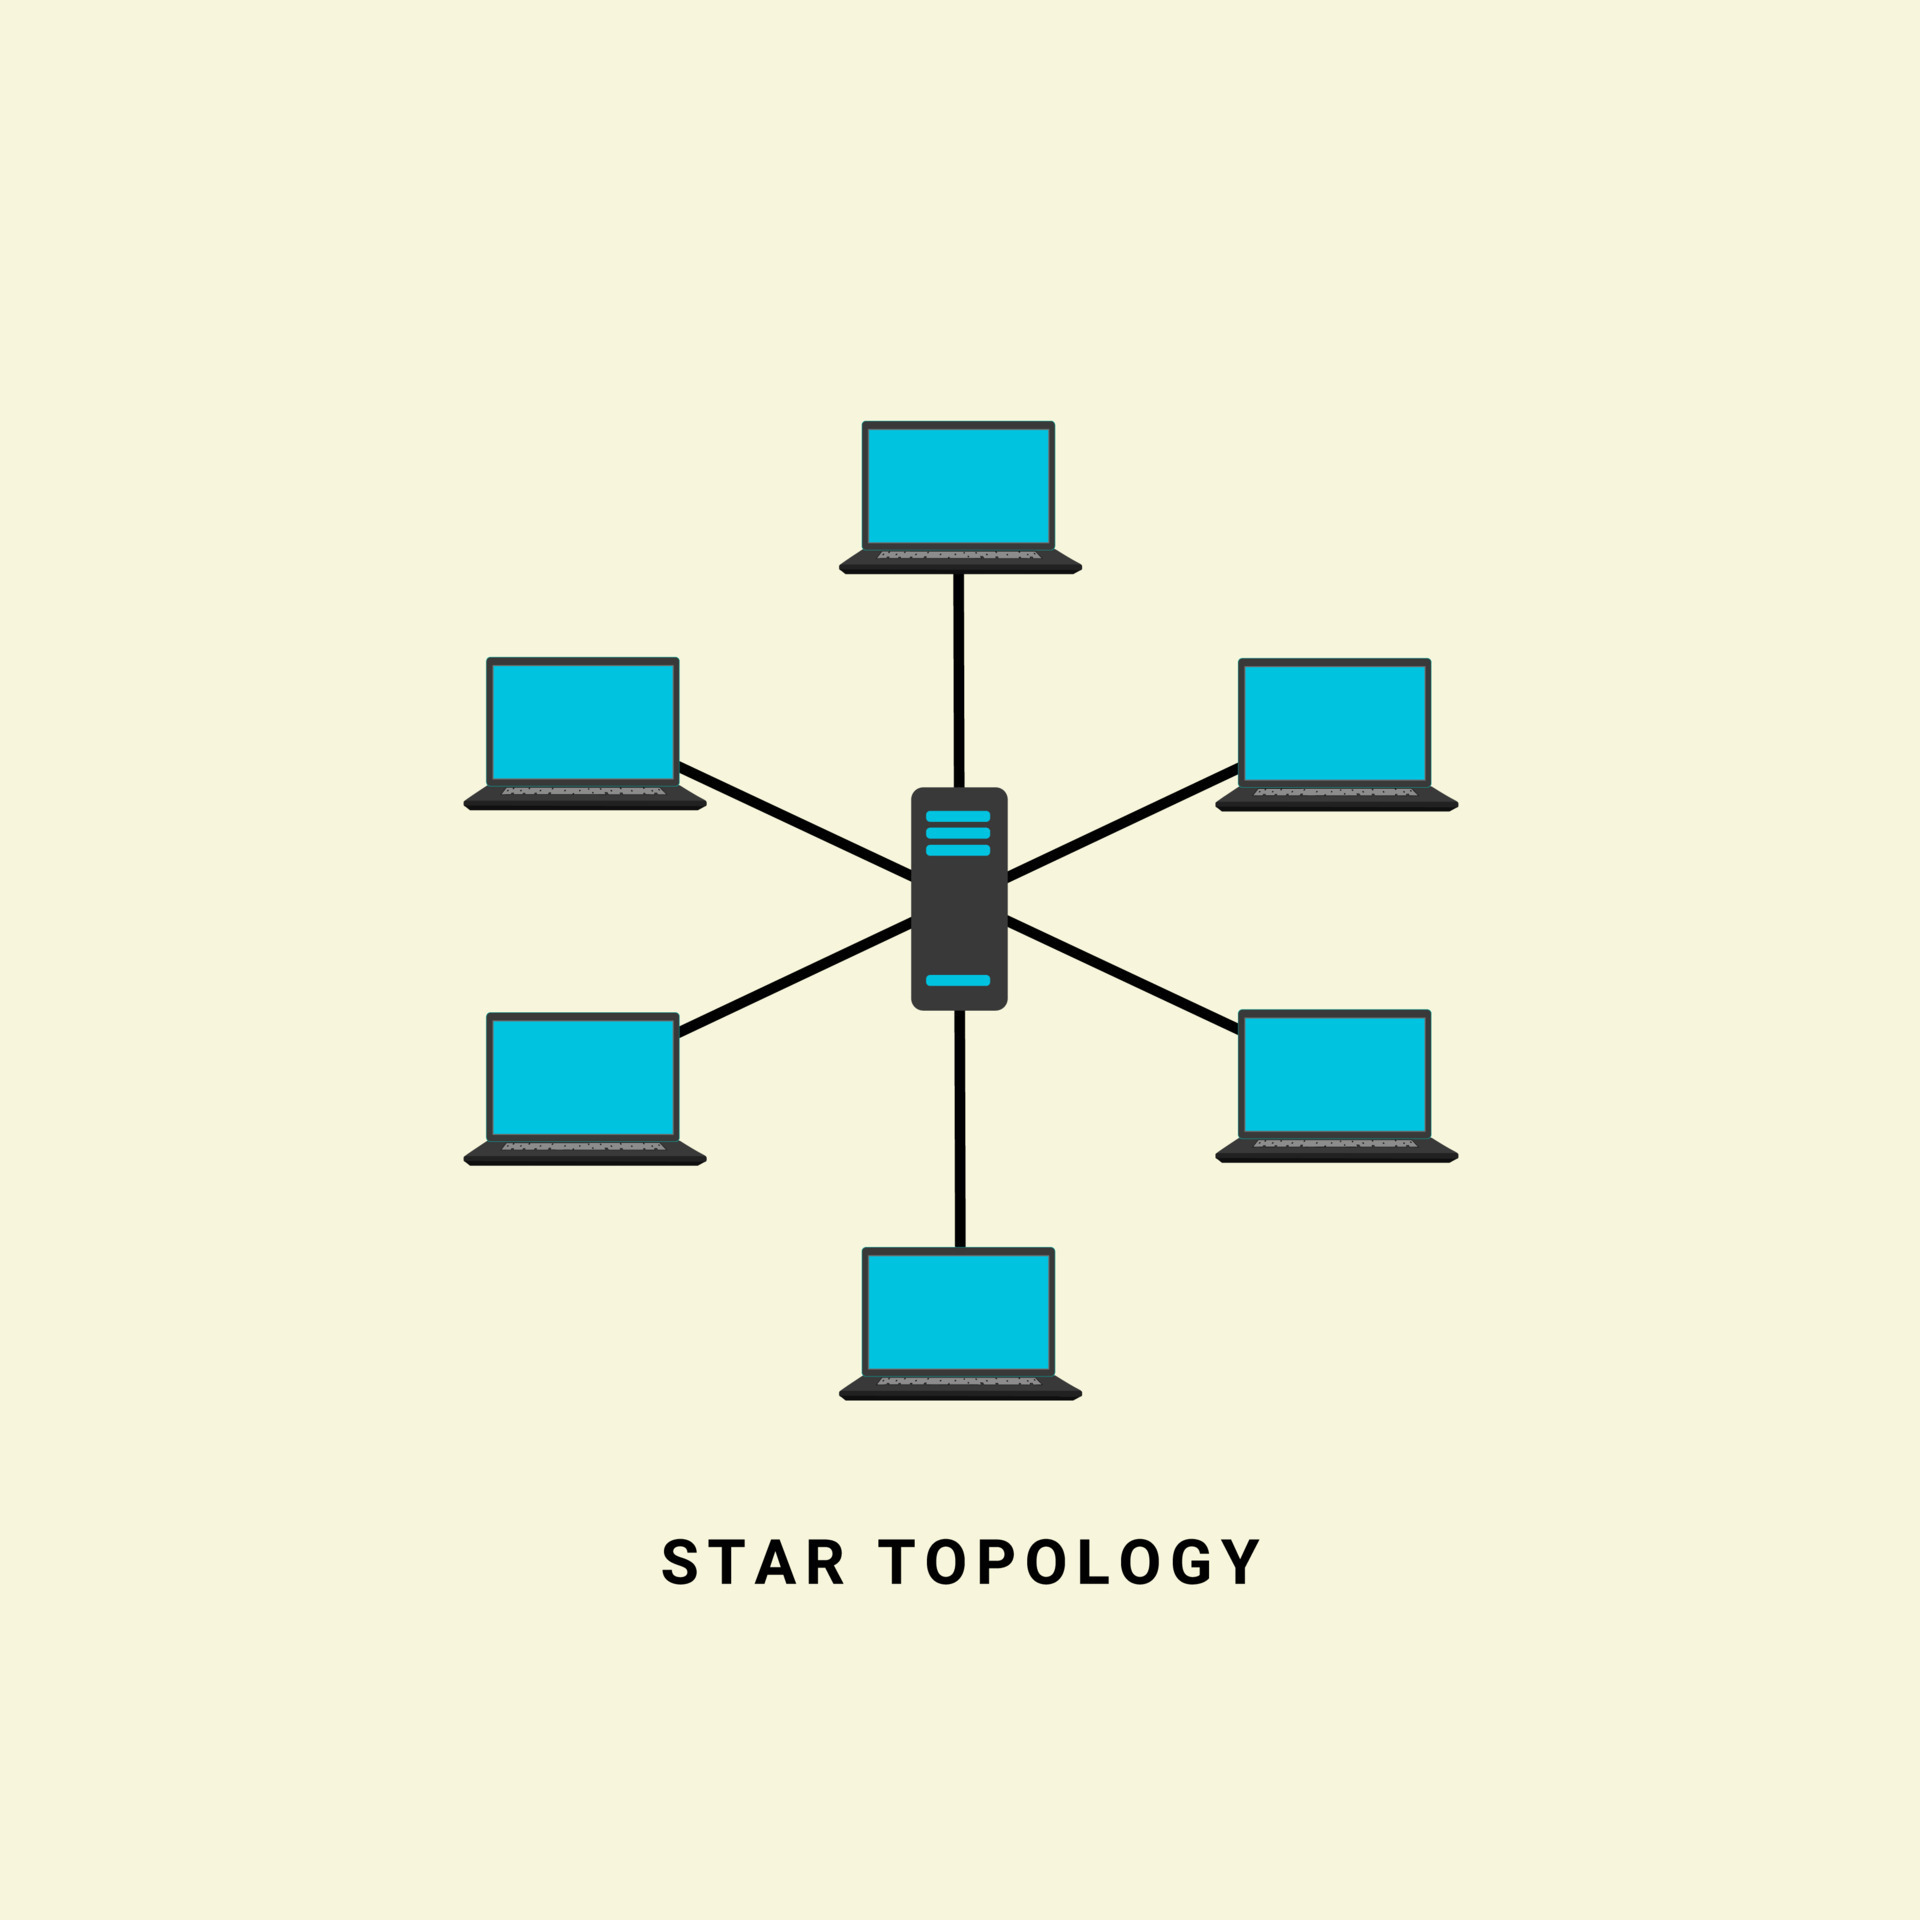
\includegraphics[width=0.6\textwidth]{images/star-topology.jpg}
  \end{figure}
\end{frame}

\begin{frame}{Torus Grid topology}
  \begin{figure}[h]
    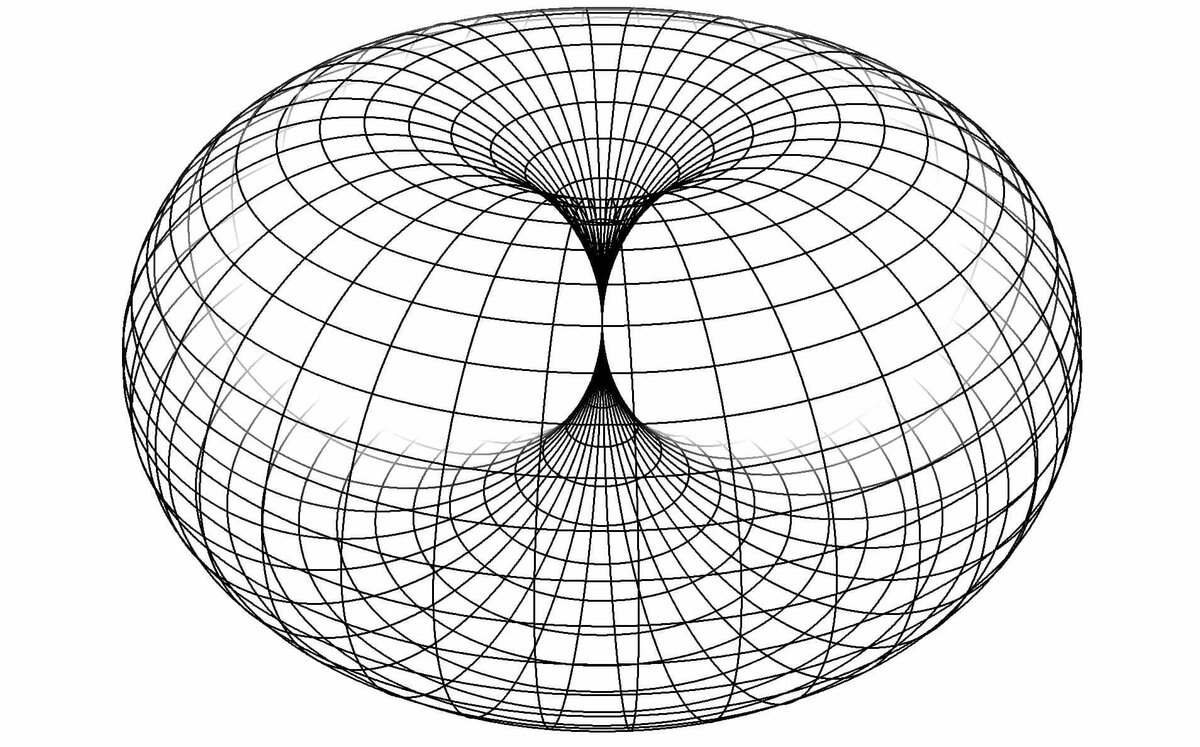
\includegraphics[width=0.4\textwidth]{images/torus.jpeg}
  \end{figure}
  \begin{figure}[h]
    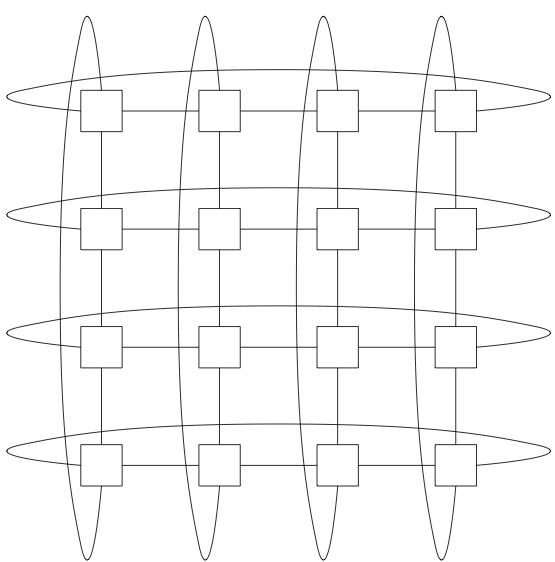
\includegraphics[width=0.4\textwidth]{images/torus-topology.png}
  \end{figure}
\end{frame}

\begin{frame}{Hypercube topology}
  \begin{figure}[h]
    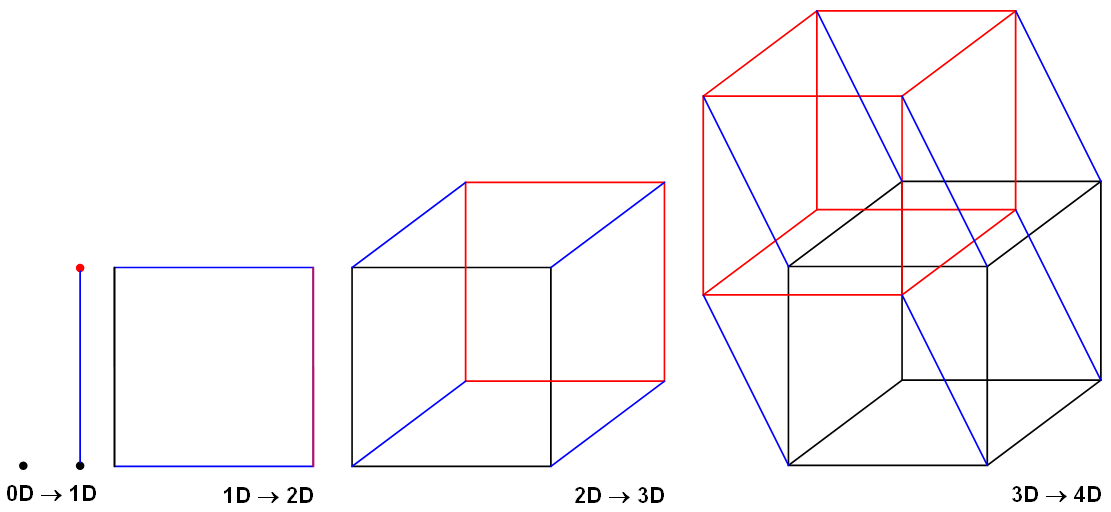
\includegraphics[width=1\textwidth]{images/hypercube-topology.png}
  \end{figure}
  Source: \href{https://en.wikipedia.org/wiki/Hypercube_internetwork_topology}{https://en.wikipedia.org/wiki/Hypercube\_internetwork\_topology}
\end{frame}

\section{Matrix Multiplication}

\begin{frame}{Matrix Multiplication}
  \begin{itemize}
    \item Horizontal Strip Scheme
    \item Vertical Strip Scheme
    \item Horizontal Strip Scheme (only matrix A partitioned)
    \item Horizontal Strip Scheme for A, Vertical Strip Scheme for B
  \end{itemize}
  Expected perf gain:
  Validate shapes (if matmul is possible for these shapes)
\end{frame}

\begin{frame}{Matrix Multiplication}
  \begin{figure}[h]
    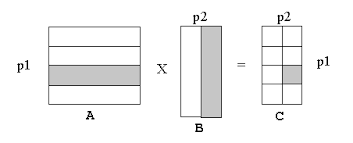
\includegraphics[width=1\textwidth]{images/matrix-multiplication.png}
  \end{figure}
\end{frame}

\section{Systems of Linear Algebraic Equations}

\begin{frame}{Systems of Linear Algebraic Equations}
  \begin{itemize}
    \item Gaussian Method - Horizontal Strip Scheme
    \item Gaussian Method - Vertical Strip Scheme
    \item Gauss-Jordan Method
    \item Iterative Methods (Jacobi)
    \item Iterative Methods (Gauss-Seidel)
    \item Simple Iteration Method
  \end{itemize}
  Generate matrix that fits conditions
  Validate:
  \begin{itemize}
    \item Determinant, ... (you can use boost library for validation step)
    \item Use data that produces only 1 solution
    \item For the last 3 tasks, check convergence conditions (otherwise there will be an infinite loop)
  \end{itemize}
  Iterative methods: max ~10\%, you can parallelize only inside iteration
\end{frame}

\section{Sort}

\begin{frame}{Sort}
  \begin{itemize}
    \item Bubble Sort (Odd-Even Transposition Sort)
  \end{itemize}
  Notes:
  \begin{itemize}
    \item Do not use std::sort for time comparison!
    \item Validation of functionality is OK
  \end{itemize}
\end{frame}

\section{Image Processing}

\begin{frame}{Image Processing}
  \begin{itemize}
    \item Image Smoothing
    \item Contrast Enhancement
  \end{itemize}
  Notes:
  \begin{itemize}
    \item Use RGB/BGR (color) linearized matrix
    \item Allowed to verify functionality using boost
    \item Compare time metric with sequential implementation
  \end{itemize}
\end{frame}

\begin{frame}
    \centering
    \Huge{Thank You!}
\end{frame}

\begin{frame}{References}
\end{frame}

\end{document}
